% ******************************************************************************
% ****************************** Custom Margin *********************************

% Add `custommargin' in the document class options to use this section
% Set {innerside margin / outerside margin / topmargin / bottom margin}  and
% other page dimensions
\ifsetCustomMargin
  \RequirePackage[left=37mm,right=30mm,top=25mm,bottom=20mm]{geometry}
  \setFancyHdr % To apply fancy header after geometry package is loaded
\fi

% *****************************************************************************
% ******************* Fonts (like different typewriter fonts etc.)*************

% Add `customfont' in the document class option to use this section

\ifsetCustomFont
  % Set your custom font here and use `customfont' in options. Leave empty to
  % load computer modern font (default LaTeX font).
  \RequirePackage{helvet}
\fi

% *****************************************************************************
% **************************** Custom Packages ********************************

\usepackage{epigraph}

%% ---- package for formatting code with line numbers
\usepackage{fancyvrb} %% for verbatim text

% **** Custom Floats ****
\usepackage{float}
\floatstyle{ruled}
\newfloat{cmd}{htb}{loc}[chapter]
\floatname{cmd}{Command}
% **** **** **** **** **** **** **** ****

%% ---- provides "\rowcolors" command
\usepackage[dvipsnames,table]{xcolor}

\usepackage{colortbl}

\usepackage{ctable}

\usepackage{subcaption}

% ---- the following package call ensures that floats will not pass a section boundary ----
\usepackage[section]{placeins}
% ---- insert �\FloatBarrier� at places that floats should not move past, perhaps at every �\section�.

% ---- if I want to extract LaTeX formulas, for instance, 
% ---- to convert them into other picture formats from pdf
%\usepackage[active,tightpage]{preview}
% ---- use \begin{preiview} ... \end{preview}

\usepackage{relsize}
\renewcommand\RSsmallest{4pt}

%------ the following package can be used for Word Review function mimicking comments ----------%
\usepackage[textsize=tiny]{todonotes} % specify ``disable'' to turn off all notes
\usepackage{setspace}
\newcommand{\note}[2][] {\todo[caption={#2}, #1] {\begin{spacing}{0.8}#2\end{spacing}}}

\usepackage{pdflscape}

% ---- for verbatim in captions. Usage: \cprotect\caption{...} ----
\usepackage{cprotect} 


% ************************* Algorithms and Pseudocode **************************

%\usepackage{algpseudocode}


% ********************Captions and Hyperreferencing / URL **********************

% Captions: This makes captions of figures use a boldfaced small font.
%\RequirePackage[small,bf]{caption}

\RequirePackage[labelsep=space,font=small,labelfont=bf,tableposition=top]{caption}
\DeclareCaptionLabelFormat{continued}{#1 #2 continued} 
\captionsetup[ContinuedFloat]{labelformat=continued}
\renewcommand{\figurename}{Fig.} %to support older versions of captions.sty
\usepackage{varioref}

\hypersetup{%
colorlinks=true,% 
citecolor=black,% 
linkcolor=black,
urlcolor=blue% 
}



% *************************** Graphics and figures *****************************

%\usepackage{rotating}
%\usepackage{wrapfig}

% Uncomment the following two lines to force Latex to place the figure.
% Use [H] when including graphics. Note 'H' instead of 'h'
%\usepackage{float}
%\restylefloat{figure}

% Subcaption package is also available in the sty folder you can use that by
% uncommenting the following line
% This is for people stuck with older versions of texlive
%\usepackage{sty/caption/subcaption}
\usepackage{subcaption}

% ********************************** Tables ************************************
\usepackage{booktabs} % For professional looking tables
\usepackage{multirow}

%\usepackage{multicol}
%\usepackage{longtable}
%\usepackage{tabularx}


% ***************************** Math and SI Units ******************************

\usepackage{amsfonts}
\usepackage{amsmath}
\usepackage{amssymb}
\usepackage{siunitx} % use this package module for SI units


% ******************************* Line Spacing *********************************

% Choose linespacing as appropriate. Default is one-half line spacing as per the
% University guidelines

%\usepackage{setspace} % already loaded
% \doublespacing
% \onehalfspacing
% \singlespacing
% \setstretch{<baselinestretch>}

% e. g.:
%\begin{spacing}{1.2}
%\tableofcontents
%\listoffigures
%\listoftables
%\end{spacing}
\raggedbottom % leaves empty space at the bottom of pages if necessary


% ************************ Formatting / Footnote *******************************

% Don't break enumeration (etc.) across pages in an ugly manner (default 10000)
%\clubpenalty=500
%\widowpenalty=500

%\usepackage[perpage]{footmisc} %Range of footnote options


% *****************************************************************************
% *************************** Bibliography  and References ********************

%\usepackage{cleveref} %Referencing without need to explicitly state fig /table

% Add `custombib' in the document class option to use this section
\ifuseCustomBib
   \RequirePackage[square, sort, numbers, authoryear]{natbib} % CustomBib

% If you would like to use biblatex for your reference management, as opposed to the default `natbibpackage` pass the option `custombib` in the document class. Comment out the previous line to make sure you don't load the natbib package. Uncomment the following lines and specify the location of references.bib file

%\RequirePackage[backend=biber, style=numeric-comp, citestyle=numeric, sorting=nty, natbib=true]{biblatex}
%\bibliography{References/references} %Location of references.bib only for biblatex

\fi

% changes the default name `Bibliography` -> `References'
\renewcommand{\bibname}{References}


% *****************************************************************************
% *************** Changing the Visual Style of Chapter Headings ***************
% This section on visual style is from https://github.com/cambridge/thesis

% Uncomment the section below. Requires titlesec package.

%\RequirePackage{titlesec}
%\newcommand{\PreContentTitleFormat}{\titleformat{\chapter}[display]{\scshape\Large}
%{\Large\filleft{\chaptertitlename} \Huge\thechapter}
%{1ex}{}
%[\vspace{1ex}\titlerule]}
%\newcommand{\ContentTitleFormat}{\titleformat{\chapter}[display]{\scshape\huge}
%{\Large\filleft{\chaptertitlename} \Huge\thechapter}{1ex}
%{\titlerule\vspace{1ex}\filright}
%[\vspace{1ex}\titlerule]}
%\newcommand{\PostContentTitleFormat}{\PreContentTitleFormat}
%\PreContentTitleFormat


% ******************************************************************************
% ************************* User Defined Commands ******************************
% ******************************************************************************

% *********** To change the name of Table of Contents / LOF and LOT ************

%\renewcommand{\contentsname}{My Table of Contents}
%\renewcommand{\listfigurename}{My List of Figures}
%\renewcommand{\listtablename}{My List of Tables}


% ********************** TOC depth and numbering depth *************************

\setcounter{secnumdepth}{2}
\setcounter{tocdepth}{2}


% ******************************* Nomenclature *********************************
 
% To change the name of the Nomenclature section, uncomment the following line

%\renewcommand{\nomname}{Symbols}


% ********************************* Appendix ***********************************

% The default value of both \appendixtocname and \appendixpagename is `Appendices'. These names can all be changed via:

%\renewcommand{\appendixtocname}{List of appendices}
%\renewcommand{\appendixname}{Appndx}

% ******************************** Draft Mode **********************************

% Uncomment to disable figures in `draftmode'
%\setkeys{Gin}{draft=true}  % set draft to false to enable figures in `draft'

% These options are active only during the draft mode
% Default text is "Draft"
%\SetDraftText{DRAFT}

% Default Watermark location is top. Location (top/bottom)
%\SetDraftWMPosition{bottom}

% Draft Version - default is v1.0
%\SetDraftVersion{v1.1}

% Draft Text grayscale value (should be between 0-black and 1-white)
% Default value is 0.75
%\SetDraftGrayScale{0.8}


%% Todo notes functionality
%% Uncomment the following lines to have todonotes.

%\ifsetDraft
%	\usepackage[colorinlistoftodos]{todonotes}
%	\newcommand{\mynote}[1]{\todo[author=kks32,size=\small,inline,color=green!40]{#1}}
%\else
%	\newcommand{\mynote}[1]{}
%	\newcommand{\listoftodos}{}
%\fi

% Example todo: \mynote{Hey! I have a note}

%%******************************** Glossary ***************************************************
%% *** \usepackage[toc,acronym]{glossaries}
% suppress page number list in glossary:
%\usepackage[nonumberlist]{glossaries}

%
% -- put the following code into a .latexmkrc file in the directory from where you run Latexmk --
%
%# add glossary generation to LATEXMK routine
%# ==========================================
%# taken from:
%# http://tex.stackexchange.com/questions/1226/how-to-make-latexmk-use-makeglossaries
%
%add_cus_dep('glo', 'gls', 0, 'run_makeglossaries');
%add_cus_dep('acn', 'acr', 0, 'run_makeglossaries');
%
%sub run_makeglossaries {
%  if ( $silent ) {
%    system "makeglossaries -q $_[0]";
%  }
%  else {
%    system "makeglossaries $_[0]";
%  };
%}
%
%push @generated_exts, 'glo', 'gls', 'glg';
%push @generated_exts, 'acn', 'acr', 'alg';
%$clean_ext .= ' %R.ist %R.xdy';

\makeglossaries

\renewcommand*{\glstextformat}[1]{\textsf{#1}}
%\renewcommand*{\glshyperlink}[1]{\textsf{#1}}

%--------------
% Glossary
%--------------
\newglossaryentry{fragment}{name=fragment, description={not a PCR duplicate. With paired reads from standard RAD (i. e. including random shearing of restriction fragments) typically identified by having different PE read sequences or different insert sizes after read mapping against a reference}}
\newglossaryentry{RAD tag}{name=RAD tag, description={genetic marker from RAD sequencing; the sequence up or downstream of a restriction site}}
\newglossaryentry{barcode}{name=barcode, description={short DNA sequence incorporated into adapter oligonucleotides that becomes part of the sequence read. Barcodes are used in order to be able to pool the DNA of different individuals, populations, treatments, etc. into one library that can be sequenced on one lane of an illumina flow cell}}
\newglossaryentry{index}{name=index, description={similar to barcode and serves the same purpose; generally incorporated into the centre of the adapter so that special sequencing run for the index is required} }
%\newglossaryentry{SbfI}{name=SbfI, description={restriction enzyme with the recognition sequence 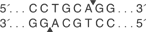
\includegraphics[scale=.5]{Sbf-I-cutsite_1_v1_000015}} }
\newglossaryentry{SbfI}{name=SbfI, description={restriction enzyme with the recognition sequence CCTGCA$\downarrow$GG} }
\newglossaryentry{XhoI}{name=XhoI, description={restriction enzyme with the recognition sequence C$\downarrow$TCGAG} }
\newglossaryentry{heterochromatin}{name=heterochromatin, description={Chromatin that remains in a highly condensed state throughout the cell cycle}}
\newglossaryentry{contig}{name=contig, description={longer consensus sequence derived from assembling smaller overlapping sequence reads}}
\newglossaryentry{linked RAD tag site}{name=linked RAD tag site, description={position in the reference sequence with at least one \gls{concordant} read pair on each side of a putative restriction site and the SE reads overlapping each other as expected from the restriction enzyme}}
\newglossaryentry{proper pair}{name=proper pair, description={read pair from illumina paired-end sequencing that got mapped to a reference in the correct orientation within a maximum expected distance from each other that is determined by the fragment size selection during the sequencing library preparation. Also called a \gls{concordant}ly mapping pair}}
\newglossaryentry{kmer}{name=kmer, description={subsequence with a specified length (k) of a longer sequence}}
\newglossaryentry{e-value}{name=Expect (E) value, description={The Expect value (E) is a parameter that describes the number of hits one can "expect" to see by chance when searching a database of a particular size}}
\newglossaryentry{read}{name=read, description={any sequence that comes out of the sequencer}}
\newglossaryentry{edit distance}{name=edit distance, description={minimum number of operations (one symbol insertion, deletion or substitution) required to change one string of symbols into another. Also known as \emph{Levenshtein distance}}}
\newglossaryentry{Ct}{name={C$_{t}$}, description={PCR cycle when a certain fluorescent threshold is reached}}
\newglossaryentry{mqs}{name={mapping quality score}, description={The mapping quality score \emph{Q} is the Phred transformation of the estimate of the probability \emph{p} that the reported mapping position does not correspond to the read's true point of origin: $Q = -10 \log_{10} p$. The way \emph{p} is estimated is different for each mapping programme, but in any case a mapping quality score \emph{Q} of 3 roughly corresponds to a mis-mapping probability \emph{p} of 0.5, i. e. the read has an estimated 50\% chance to have derived from a location other than the one reported}}
\newglossaryentry{discordant}{name=discordant, description={A read pair is called discordant if it aligns without the expected relative mate orientation (here: forward--reverse or reverse--forward) or outside the expected range of distances between mates. Note that \texttt{bowtie2} only calls discordant read pair mappings if both reads map \emph{uniquely}. Here, I am NOT adopting this requirement}}
\newglossaryentry{concordant}{name=concordant, description={A read pair is called concordant if it aligns with the expected relative mate orientation (here: forward--reverse or reverse--forward) and within the expected range of distances between mates. This is also called a \gls{proper pair}. The complement of \gls{discordant}}}
\newglossaryentry{Levenshtein distance}{name=Levenshtein distance, description={The Levenshtein distance is equal to the minimum number of operations (edits) required to transform one string into another. The allowed operations are single character insertions, deletions and substitutions. This is also known as edit distance.}}
\newglossaryentry{all pairs}{name={all pairs}, description={all the pairs of sequences below a given Levenshtein distance are identified during the graph construction phase}}
\newglossaryentry{transitive clusters}{name=transitive clusters, description={Two read clusters are merged if the distance of any pair of reads between the clusters is below threshold. After merging, the newly created cluster can contain read pairs with distance above the clustering threshold}}
\newglossaryentry{graph}{name=graph, description={A network of connected sequences. Two sequences are directly connected if they match with distance below a threshold. The distance is a measure of the strength of connection, aka "edge weight". Graphs can be stored as a list of pairs of sequences, with an optional edge weight. All graphs here should be "undirected cyclic graphs"}}
\newglossaryentry{Nmer}{name=\emph{N}mer, description={synonymous to kmer, unit, word; a subsequence of size \emph{N} that is overlapping or contiguous with the next subsequence of size \emph{N} and stored in a dictionnary (aka hash) for fast lookup}}
\newglossaryentry{population allele frequency}{name=population allele frequency, description={The population allele frequency is the (unknown) frequency of the allele in the entire population}}
\newglossaryentry{sample allele frequency}{name=sample allele frequency, description={The sample allele frequency is the frequency of the allele among the individuals in a specific sample}}
\newglossaryentry{connected component}{name=connected component, description={All nodes (here sequence reads) after all--pairs search (and before clustering!) that are directly connected by an edge or indirectly connected via several nodes belong to the same connected component} }

%----------------
% Acronyms
%----------------
\newacronym{snp}{SNP}{single nucleotide polymorphism}
\newacronym{rad}{RAD}{Restriction Site associated DNA}
\newacronym{pe}{PE}{paired-end}
\newacronym{se}{SE}{single-end}
\newacronym{bp}{bp}{base pair}
\newacronym{Mbp}{Mbp}{mega base pairs}
\newacronym{Gbp}{Gbp}{giga base pairs}
\newacronym{indel}{indel}{small sequence insertion or deletion polymorphism}
\newacronym{SAM}{SAM}{Sequence Alignment/Map format}
\newacronym{EST}{EST}{expressed sequence tag}
\newacronym{ddRAD}{ddRAD}{double digest RAD}
\newacronym{ML}{ML}{maximum likelihood}
\newacronym{SFS}{SFS}{site frequency spectrum}
\newacronym{HWE}{HWE}{Hardy Weinberg equilibrium}
\newacronym{CI}{CI}{confidence interval}
\newacronym{EM}{EM}{Expectation Maximisation}
\newacronym{DEM}{DEM}{digital elevation model}
%\usepackage[toc]{glossaries}
%\makeglossaries
%\renewcommand*{\glstextformat}[1]{\textsf{#1}}
%
%\newglossaryentry{fragment}{name=fragment, description={not a PCR duplicate}}
%
%\newacronym{snp}{SNP}{single nucleotide polymorphism}

%% ******************************** SVG *************************************
%\newcommand{\executeiffilenewer}[3]{%
%	\ifnum\pdfstrcmp{\pdffilemoddate{#1}}%
%	{\pdffilemoddate{#2}}>0%
%	{\immediate\write18{#3}}\fi%
%}
%\newcommand{\includesvg}[1]{%
%	\executeiffilenewer{#1.svg}{#1.pdf}%
%	{./inkscape -z -D -f #1.svg %
%	--export-pdf=#1.pdf --export-latex}%
%	\import{./Figs/Inkscape_Graphics}{#1.pdf_tex}%
%}

